\documentclass{article}
\usepackage{graphicx}
\usepackage{geometry}
\usepackage{mathtools}
\usepackage{wrapfig}
\usepackage{lipsum}
\usepackage[dvipsnames]{xcolor}
\usepackage{multicol}
\usepackage[italian]{babel}
\usepackage{wrapfig}
\usepackage{hyperref}
\usepackage{listings}
\usepackage{xcolor}
\hypersetup{
    colorlinks=true,
    linkcolor=blue,
    pdftitle={Ingegneria degli algoritmi},
    }

\geometry{a4paper, top=2.5cm, bottom=2.5cm, left=3cm, right=3cm}




\definecolor{codegreen}{rgb}{0,0.6,0}
\definecolor{codegray}{rgb}{0.5,0.5,0.5}
\definecolor{codepurple}{rgb}{0.58,0,0.82}
\definecolor{backcolour}{rgb}{0.95,0.95,0.92}
\definecolor{bleudefrance}{rgb}{0.19, 0.55, 0.91}
\definecolor{aliceblue}{rgb}{0.94, 0.97, 1.0}
\lstdefinestyle{mystyle}{    
	language=C, 
    commentstyle=\color{codegreen},
    keywordstyle=\color{bleudefrance},
    numberstyle=\tiny\color{codegray},
    stringstyle=\color{codepurple},
    basicstyle=\ttfamily\footnotesize,
    breakatwhitespace=false,         
    breaklines=true,                 
    captionpos=b,                    
    keepspaces=true,                 
    numbersep=5pt,                  
    showspaces=false,                
    showstringspaces=false,
    showtabs=false,                  
    tabsize=2
    }

\lstset{style=mystyle}




\title{\textbf{Ingegneria degli Algoritmi}}
\author{Nicolò Bianchi e David Julian Belfiori }
\date{ }

\def\setupqm{\catcode`\?=13 }
\begingroup
\catcode`\?=13
\gdef?{\hphantom{0}}
\endgroup

\setlength{\columnsep}{0.5cm}

\begin{document}
\maketitle
\tableofcontents
\newpage

\section{Introduzione}
\subsection{Che cosa è un algoritmo}
Un algoritmo è una procedura per risolvere un problema ,ovvero produrre una risposta a partire dai dati che abbiamo ricevuto in input.
Un algoritmo deve rispettare determinate caratteristiche:
\begin{itemize}
    \item Definitezza (nessuna ambiguità)
    \item Input
    \item Output
    \item Finitezza
    \item Efficacia (ogni passo deve poter esser eseguito in un tempo finito)
\end{itemize}
riprendendo l'ultimo punto,  per definizione di algoritmo, esso deve rispondere (produrre un output) in un tempo finito, altrimenti stiamo parlando di un metodo compuazionale.\\

\textbf{N.B} per ogni problema non esiste un solo algoritmo che lo risolve, non appena si dimostra che l'insieme degli algoritmi che risolvono il problema non è vuoto, si apre la discussione quale sia il 'migliore'
\subsection{Come si valuta un algoritmo}
Si può valutare la qualità di un algoritmo descrivendone:
\begin{itemize}
    \item \textbf{Complessità temporale} : il tempo \textbf{T(n)} impiegato per risolvere un problema di dimensione n 
    \item \textbf{Complessità spaziale}: la quantità di memoria impiegata \textbf{S(n)} per risolvere un problema di dimensione n 
\end{itemize}
\section{Corretteza degli algoritmi}
Per qualunque algoritmo di deve dimostrare la terminazione (in un tempo finito) e la \textit{correttezza}.
In informatica per verificare la correttezza di un algoritmo spesso si dimostra per induzione utilizzando degli invarianti \footnote{Le invarianti di ciclo sono un utile strumento che permette di provare la correttezza e la terminazione di un algoritmo che esegue al suo interno cicli.}.
\\
\\
Es. Procedura Minsearch

\begin{wrapfigure}{l}{0.5\textwidth}
  \centering
  
  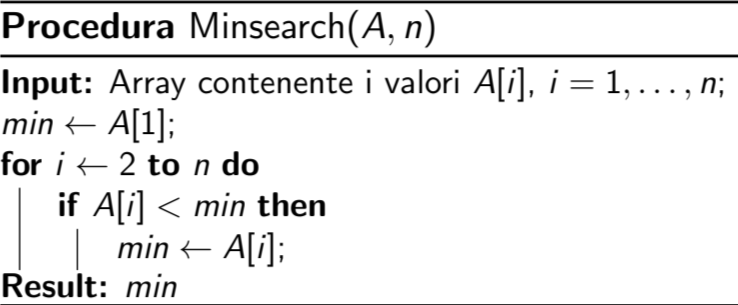
\includegraphics[width=0.5\textwidth]{photo/Minsearch.png}
 
\end{wrapfigure}
    
\textbf{Dimostrazione di corretezza}
\begin{enumerate}
    \item prima dell'inizio consideriamo solo il vettore A[1:1](che contiene solo un elemento), e la var. min è inizializzata bene.
    \item All'iterazione i diamo per vero che \textit{min} contenga il minimo del vettore A[1:i-1], allora considerando il valore A[i] ci sono due possibilità, che \(A[i]<\textit{min}\) oppure no, in ogni caso \textit{min} contiene il minimo valore del vettore A[1:i], ossia la proprieta invariante che volevamo.
\end{enumerate}
\newpage
\section{Complessità computazionale}
Per risolvere un problema, spesso sono disponibili molti algoritmi diversi. Un criterio per scegliere il migliore consiste nel valutare la 'bontà' di un algoritmo in base alla quantità di risorse utilizzate (tempo e spazio) per il calcolo.
\subsection{Quanto costa risolvere un problema?}
In pratica, non è possibile misurare il tempo di calcolo di un algoritmo con il numero di secondi richiesti per eseguire una determinata procedura.
Infatti tale tempo è fortemente dipendente dai dati in ingresso, dal linguaggio in cui la procedura è descritta e dalla natura e la velocità del calcolatore elettronico. \\
Poichè i problemi hanno una dimensione che dipende dalla grandezza dei dati in ingresso, il tempo di calcolo si può esprimere come il costo complessivo delle operazioni elementari (aritmetiche, logiche, di confronto e di assegnazione)  in funzione della dimensione \textit{n} dei dati di ingresso
\paragraph{E' se la dimensione \textit{n} non è sufficiente a determinare completamente il tempo di esecuzione?}
\subparagraph{Il costo delle operazioni è principalmente valutato in 3 casi:}
\begin{enumerate}
    \item \textbf{Worst case:} \(T(n)\) è  \(O(f(n))\) \textbf{per qualunque} input possibile di dimensione \textit{n}
    \item \textbf{Average case:} \(T(n)\) è  \(\Theta(f(n))\) \textbf{in media} su tutti gli input possibili di dimensione \textit{n}
    \item \textbf{Best case:} \(T(n)\) è  \(\Omega (f(n))\) questo valore viene raggiunto \textbf{per alcuni} degli input di dimensione \textit{n}
\end{enumerate}
\subparagraph{Casi comuni:}
\begin{enumerate}
\item \(O(1)\) : algoritmo che richiede un tempo costante
\item\(O(log(n))\): algoritmo di ordine logaritmico
\item\(O(n)\): algoritmo di ordine lineare
\item\(O(n^k)\): algoritmo di ordine polinomiale 
\item\(O(a^n)\): algoritmo di ordine esponenziale
\end{enumerate}
Gli algoritmi di \textbf{complessità polinomiale} sono \textbf{considerati inefficienti} e non sono accettabili. Una volta realizzato un algoritmo con complessità polinomiale, si cerca di migliorarne le prestazioni progettando algoritmi con complessità sempre inferiore  \\
\\
\textbf{Esempio: }un semplice algoritmo polinomiale è il \textit{Selection Sort}, che è basato sulla proprietà che in una sequenza ordinata il primo elemento ha valore minimo
\subsection{Problemi vs Algoritmi}

Inanzi tutto distinguiamo la \textbf{complessità di un algoritmo} e la \textbf{complessità di un problema}
\begin{itemize}
    \item \textbf{Complessità di un algoritmo} è la complessità di un particolare metodo per la soluzione di un problema
    \item \textbf{Complessità di un problema} è la complessità del \textbf{migliore} algoritmo che risolve quel problema 
\end{itemize}
Ad esempio, l'ordinamento per inserzione è un algoritmo di ordine \(O(n^2)\) mentre il problema dell'ordinamento per confronti ammette una soluzione in tempo \(O(nlog(n))\)
\newpage
\textbf{Esempio:} Insertion Sorting (ordinamento per inserzione)
\begin{figure}[h]
    \centering
    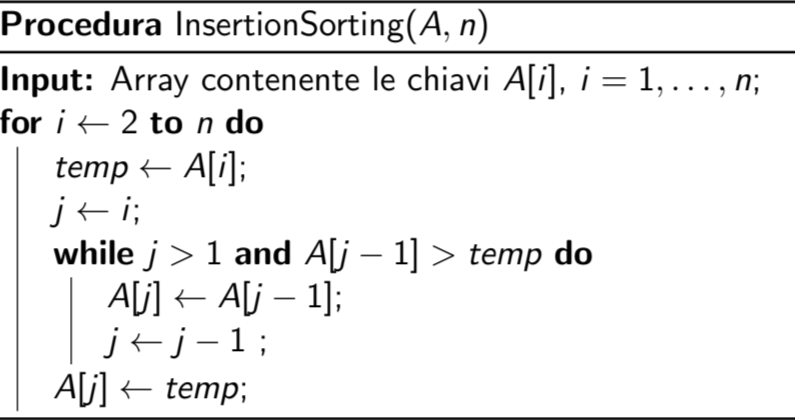
\includegraphics[width=0.5\linewidth]{photo/InsertionSorting.png}
\end{figure}
Data una procedura, si valuta il costo del suddetto algoritmo attraverso delle "linee guida":
\begin{itemize}
    \item le espressioni scalari \footnote{Qualsiasi entità numerica a cui corrisponda unicamente un valore e non una direzione} elementari hanno costo O(1)
    \item il costo di una sequenza di istruzioni è dato dalla somma dei costi delle singoli istruzioni 
    \item il costo di un ciclo è la somma del costo delle singole iterazioni sull'insieme di tutte le iterazioni
    \item un istruzione condizionale (if) ha un costo nel \textbf{caso peggiore} che è il massimo tra i costi del ramo \textit{if} e del ramo \textit{else}; per il costo medio occorre fare la media pesata (con la stima delle probabilità che esca un caso o un altro 
\end{itemize}
\subsection{Costo di un ciclo}

Per un ciclo bisogna calcolare: 
\begin{equation}
   \sum_{i \in I} C(i)
\end{equation}
Dove:
\begin{itemize}
    \item \textit{i} è un iterazione
    \item \textit{I} è l'insieme di tutte le iterazioni
    \item \textit{C(i)} è il costo della i-esima iterazione 
\end{itemize}
Spesso il costo di un ciclo è costante, trovare l'insieme di tutte le iterazioni I è facile nei ciclo \textit{for} , ma non necessariamente nei cicli \textit{while} 
\\
\textbf{N.B} A cicli innestati corrispondono somme multiple 
\begin{figure}[h]
    \centering
    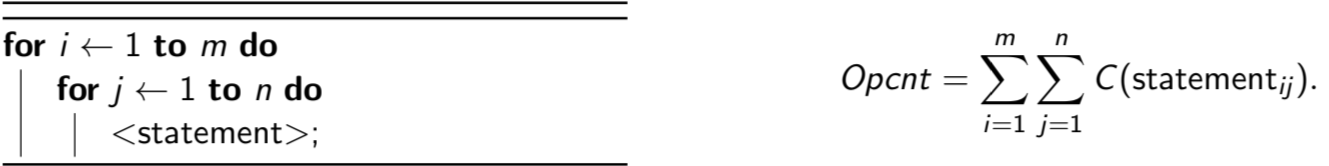
\includegraphics[width=0.75\linewidth]{photo/costo_ciclo_annidato.png}
\end{figure}
\newpage
\subsection{Complessità computazionale InsertionSorting}
\begin{figure}[h]
  \centering
  
  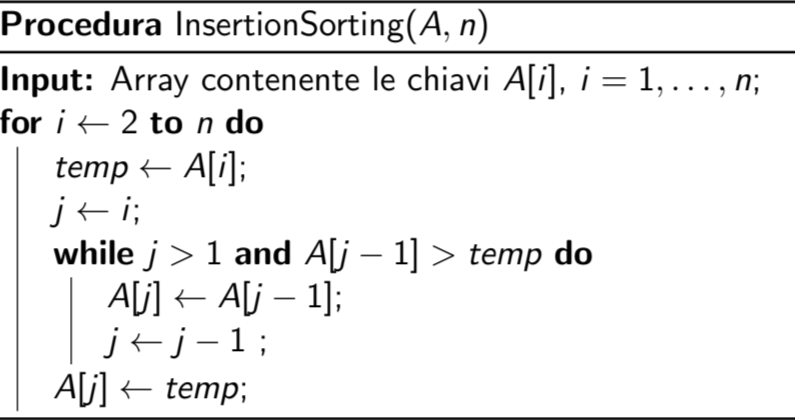
\includegraphics[width=0.5\textwidth]{photo/InsertionSorting.png}


\end{figure}
Per il ciclo interno \textit{while}:
 \begin{itemize}
     \item Nel caso migliore, esegue il controllo ed esce immediatamente (nel caso migliore sarà lineare)
     \item nel caso peggiore viene eseguito \textit{i}-1 volte
 \end{itemize}
 Abbiamo quindi una complessità \(\Omega(n)\) o \(O(n^2)\)

\subsection{Complessità computazionale BinarySearch}
\begin{figure}[h]
  \centering
  
  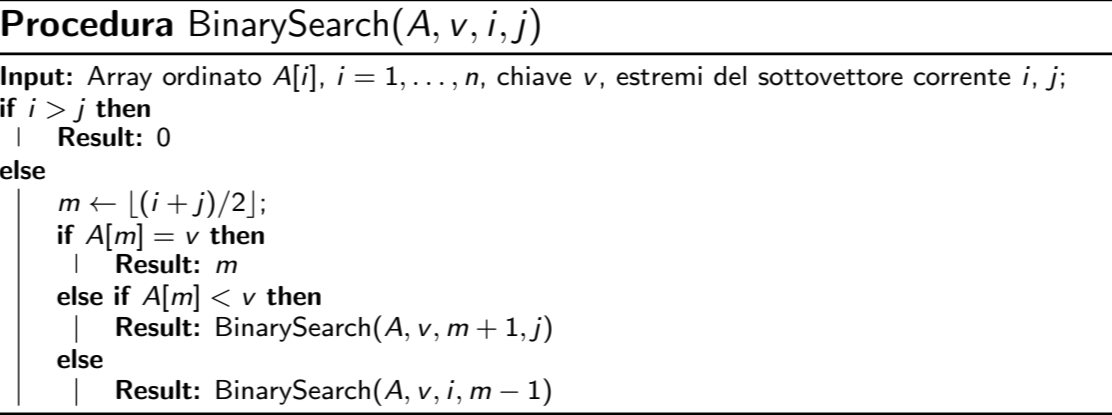
\includegraphics[width=0.75\textwidth]{photo/BinarySearch.png}
\end{figure}
Al primo passo la dimensione del vettore è \textit{n} , ad ogni passo la dimensione si dimezza , nel caso peggiore è quindi necessario eseguire un numero di passi \textit{k} tale che 
\begin{equation}
    n/2^k \le 1 \xrightarrow{} k \ge \log_{2}(n)
\end{equation}
La procedura di \textbf{BinarySearch} è quindi è di \textbf{ordine \(O(\log(n)\)}
\subsection{Funzione Ricorsiva}

In una funziona ricorsiva ciascuna istanza applicata ad un problema è di dimensione \textit{n}=1 (di cui possiamo calcolare il costo separatamente), oppure suddividere il suddetto problema di dimensione \textit{n} in sotto problemi di dimensione più piccola, le cui soluzioni saranno poi combinate per costituire la soluzione complessiva  
\\
nell'analisi delle funzioni ricorsive si usano spesso delle relazioni di ricorrenza ,ossia delle equazioni del tipo
    \begin{equation}
        T(n)=G(T(n-n_1),T(n-n_2),T(n-n_3),...T(n-n_k)
    \end{equation}
Ci sono due tipi di ricorrenze :
\begin{itemize}
    \item Lineari a termini costanti.
       \begin{itemize}
           \item Una ricorrenza a termini lineari sarà del tipo
\begin{equation}
    T(n)=(\sum _{i=1} ^{k} a_iT(n-i)) + cn^\beta \;\;\;\;\;   n > k
\end{equation}
       \end{itemize}
    \item A partizione bilanciata : dove si divide il problema principale di dimensione \textit{n} in un insieme di sotto problemi di dimensione \(n/b\), le cui soluzioni vengono ricombinate per costruire la soluzione complessiva 
\end{itemize}
    \begin{equation}
       T(n)= \begin{cases}
            1  & \text{se n=1}\\
            aT(\frac{n}{b})+n^\beta & se \; \; n>1
       \end{cases}
    \end{equation}

Il termine \(n^\beta\) misura il costo per suddividere il problema in sotto problemi e ricomporre le loro soluzioni 

\section{Nozioni base di C}
\subsection{Variabili}
Ad ogni variabile in C deve essere associato un tipo, quindi quando si dichiara una variabile bisogna specificare sempre di che tipo è. In C le variabili possono essere di 5 tipi base:
\begin{itemize} \label{Tipi di dato}
    \item \textbf{Int}: numeri interi a 16 bit 
    \item \textbf{Float}: sono numeri a virgola mobile 32 bit
    \item \textbf{Char}: sono le variabili che contengono un carattere 8 bit 
    \item \textbf{Double} Numeri a virgola mobile a precisone doppia 64 bit
    \item  \textbf{Void} \textit{Speciale} : le variabili void sono usate per dichiarare dei puntatori \footnote{Un puntatore è una variabile che contiene l'indirizzo di memoria di un'altra variabile (il puntatore x punta alla variabile y).} e per definire delle funzioni che non ritornano alcun valore 

\end{itemize}
\subsubsection{Regole di visibilità}
Ogni variabile ha un compito e una conseguente visibilità
\begin{itemize}
    \item Variabili globali
    \item Variabili locali
    \item Variabili statiche 
\end{itemize}
\subsubsection{Modificatori}
I modificatori sono parole chiave che appunto modificano le proprietà predefinite delle variabili int e char e sono di 4 tipi:
\begin{itemize}
    \item \textbf{Signed }: Lo specificatore signed indica che una data variabile va trattata con segno positivo o negativo, nei calcoli aritmetici. Può essere impiegato sia come modificatore di alcuni tipi base, che direttamente come tipo di dati, applicandosi in modo predefinito al tipo int
    \item \textbf{Unsigned }: Lo specificatore unsigned indica che una data variabile va trattata sempre con segno positivo, nei calcoli aritmetici.
    \item \textbf{Short} : dal nome si evince che riduce lo spazio assegnato alla variabile.\\
    Limita l'utente a memorizzare piccoli valori interi da -32768 a 32767. Può essere utilizzato solo su tipo di dati int.
    \item \textbf{Long}:  al contrario di Short aggiunge lo spazio assegnato alla variabile .\\
    Consente all'utente di memorizzare numeri molto grandi da -9223372036854775808 a 9223372036854775807
\end{itemize}
\subsection{Operatori}
Sulle variabili agiscono degli operatori per costiture dele espressioni:
\begin{itemize}
    \item \textbf{Operatore di assegnazione}: =
    \item \textbf{Operatori aritmetici}: gli usuali 
    \item \textbf{Operatori relazionali} : \(<\)  $>$  \; == \; !=
    \item \textbf{Operatori di incremento}: ++ --
    \item \textbf{Operatori logici}:$|$ $||$ $\&$ $\&\&$ 
\end{itemize}
\subsection{Strutture di controllo: Switch}
Il blocco switch-case permette di selezionare un'istruzione da eseguire in base ad una variabile.\\
 L'istruzione break interrompe l'elaborazione del blocco switch, in modo da uscire subito dal blocco se una condizione è vera. L'istruzione break è opzionale, ma se non viene usata, vengono eseguite le istruzioni dei casi seguenti.
\begin{lstlisting}[language=C]
switch (variabile)
{
 case valore1:
  // istruzione1
  break;
 
 case valore2:
  // istruzione2
  break;
 
 case valoreN:
  // istruzioneN
  break;
}
\end{lstlisting}
\subsubsection{Istruzione switch-case-default}
\begin{lstlisting}[language=C]
int main(void)
{
 int scelta;

 printf("Inserisci Una Scelta: ");
 scanf("%d", &scelta);

 switch(scelta){
        case  1: printf("Scelta 1\n");     break; 
        case  2: printf("Scelta 2\n");     break;
        case  3: printf("Scelta 3\n");     break;
        default: printf("Altra Scelta\n"); break;
 }
}
\end{lstlisting}
\newpage
\subsection{Tipi di dati derivati: Array e puntatori}
In linguaggio C, i tipi di dati derivati sono tipi di dati che vengono creati a partire dai tipi di dati primitivi (come int, float, char, ecc.) \ref{Tipi di dato}  attraverso varie operazioni. Questi tipi di dati derivati consentono di adattare e organizzare i dati in modi specifici per soddisfare le esigenze di programmazione
\subsubsection{Array}
un array è in tipo di dato aggregato costituito a molteplici dati elementari i quali
\begin{itemize}
    \item Hanno tutti lo stesso tipo base 
    \item sono identificati da un indice numerico (o da un inseme di indici)
\end{itemize}
il numero di indici è necessario per identificare un elemento e per comprendere la dimensione complessiva dell'array:  monodimensionale , bidimensionale , etc.

\begin{lstlisting}[language=C]
#inlude <stdio.h>
#define N 100
int main(int argc, char *argv[]){
    int a[N],i;

    for (i=0,i<N,i++){
        a[i]=i
    }
}
\end{lstlisting}
\label{Esempio di array monodimensionale}

\begin{lstlisting}[language =C]
#include <stdio.h>

int main() {
    // Dichiarazione di un array bidimensionale 2x2
    int arrayBidimensionale[2][2];

    // Accesso agli elementi dell'array
    arrayBidimensionale[0][0] = 1;
    arrayBidimensionale[0][1] = 2;
    arrayBidimensionale[1][0] = 3;
    arrayBidimensionale[1][1] = 4;

    // Stampa dell'intero array
    printf("Array bidimensionale:\n");
    for (int i = 0; i < 2; i++) {
        for (int j = 0; j < 2; j++) {
            printf("%d ", arrayBidimensionale[i][j]);
        }
        printf("\n");
    }

    return 0;
}
\end{lstlisting}
\label{ esempio di array bidimensionale}

\begin{itemize}
    \item il primo elemento corrisponde a [0][0] e l'ultimo a [M-1][N-1]
\end{itemize}
\newpage
\subsection{Puntatori}
Un puntatore è una variabile speciale che contiene l'indirizzo di memoria di un'altra variabile. In altre parole, anziché contenere un valore direttamente, un puntatore contiene l'informazione su dove trovare il valore in memoria. I puntatori sono un concetto fondamentale in C e sono utilizzati per lavorare con dati complessi e strutture di dati dinamiche.
\\
Esempio: come dichiarare un puntatore
\begin{lstlisting}[language =C]

int x = 10; // Dichiarazione di una variabile intera
int *ptr;   // Dichiarazione di un puntatore a un intero

ptr = &x;    // Assegna all'indirizzo del puntatore l'indirizzo di x

printf("Il valore di x: %d\n", x);
printf("Il valore a cui punta il puntatore: %d\n", *ptr);

\end{lstlisting}
L'operatore \textbf{\&} consente di ottenere l'indirizzo di memoria di un altra variabile, e quindi assegnarlo ad un puntatore.
\paragraph{Perché i puntatori hanno generalmente un tipo associato ?}

Specificare il tipo di dato a cui si riferisce il puntatore è un modo per garantire che il compilatore sappia come interpretare i dati memorizzati all'indirizzo di memoria puntato dal puntatore. Ad esempio, se si dichiara un puntatore a un intero (int), il compilatore sa che dovrebbe trattare i dati a quell'indirizzo come valori interi. 

\subsubsection{Operazioni sui puntatori}
Cosa \textbf{C} ci permette di fare con un puntatore:
\begin{itemize}
	\item Dichiarare un vettore: \verb|	type *ptr;|
	
	\item Accedere al valore puntato: \verb|val= *ptr;|
	
	\item Accedere ad un indirizzo : \verb|type *ptr= &val;|

\end{itemize}
\begin{lstlisting}[language = C]
	//Esempio: algoritmo per il calcolo del massimo comune divisore  utilizzano i puntatori
	#include <stdio.h>
	#include <stdlib.h>
	
	// utlizzio di puntatori per scambiare due variabili e le dichiaro unsigned perche non possono essere negative
	void swap(unsigned int *a,unsigned int *b){
		unsigned temp;
		temp=*a; 
		//temp prende il valore di a che a sua volta prende il valore di m e quindi temp //prende il valore di m proveniente dalla funzione MCD
		*a=*b;
		*b=temp;
	}
	
	//le dichiaro unsigned perche non possono essere negative
	unsigned int MCD(unsigned m,unsigned n){
		if (m==0 || n==0){
			printf("errore");
			exit(1);
		}
		while (m!=n){
			if (m<n){
				swap(&m,&n);
			}
			m=m-n;
		}
		return m;
	}
	
	int main(int argc, char **argv){
		unsigned int k = MCD(12, 18);
		printf("%d",k);}
	
\end{lstlisting}
\subsubsection{La funzione malloc}
La funzione malloc è utilizzata per allocare dinamicamente memoria nell'heap, consentendo al programma di gestire la memoria in modo flessibile. L'allocazione dinamica della memoria è utile quando non si conosce a priori la dimensione esatta della memoria necessaria o quando si desidera utilizzare la memoria in modo dinamico durante l'esecuzione del programma.
\\
\\
\textbf{La funzione malloc} (che sta per "memory allocation") \textbf{prende} un unico argomento, che rappresenta \textbf{il numero di byte di memoria da allocare}, e \textbf{restituisce un puntatore a un'area di memoria allocata}. Ad esempio:
\begin{lstlisting}[language =C]
	#include <stdio.h>
	#include <stdlib.h>
	
	int main() {
		int *p;
		p = (int *)malloc(sizeof(int)); // Alloca memoria per un intero (4 byte su molti sistemi)
		if (p == NULL) {
			printf("Errore di allocazione di memoria.\n");
			return 1;
		}
		
		// Ora puoi usare la variabile puntatore p per accedere alla memoria allocata dinamicamente
		
		*p = 42;
		printf("Il valore di p : %d\n", *p);
		
		// Quando hai finito di usare la memoria,e'importante deallocarla per evitare memory leak
		free(p);
		
		return 0;
	}	
\end{lstlisting}
\subsection{Strutture}
In linguaggio C, le strutture (o "struct") sono utilizzate per creare tipi di dati personalizzati che possono contenere uno o più membri di diversi tipi. Una struttura è una collezione di variabili che possono rappresentare un oggetto o una entità complessa. Ogni membro di una struttura può essere di qualsiasi tipo di dati C, compresi tipi di dati primitivi (come int, float, char) o altre strutture.
\\
Ecco come dichiarare e utilizzare una struttura in C:
\begin{lstlisting}[language =C]
	#include <stdio.h>
	
	// Dichiarazione di una struttura
	struct Student {
		char name[50];
		int age;
		float gpa;
	};
	
	int main() {
		// Dichiarazione di una variabile di tipo struct Student
		struct Student student1;
		
		// Accesso ai membri della struttura e assegnazione di valori
		strcpy(student1.name, "Alice");
		student1.age = 20;
		student1.gpa = 3.5;
		
		// Stampa dei membri della struttura
		printf("Nome: %s\n", student1.name);
		printf("Eta: %d\n", student1.age);
		printf("GPA: %.2f\n", student1.gpa);
		
		return 0;
	}
	\end{lstlisting}

\textbf{Esempio}: Un algoritmo che gestisce informazioni su persone (Joe e Frank) utilizzando strutture e funzioni.
\begin{lstlisting}[language=C]
	#include <stdio.h>
	#include <stdlib.h>
	#include <assert.h>  
	#include <string.h>
	
	// Definizione di una struttura "person" per rappresentare informazioni su una persona.
	struct person {
		char *name;      // Nome della persona
		int age;         // Eta'della persona
		float height;    // Altezza della persona
		float weight;    // Peso della persona
	};
	
	// Funzione per creare una nuova persona e restituire un puntatore a essa.
	struct person *person_create(char *name, int age, float height, float weight) {
		struct person *who = malloc(sizeof(struct person)); // Alloca memoria per una persona
		assert(who != NULL); // Assicurati che l'allocazione di memoria sia riuscita
		who->name = strdup(name); // Copia il nome nella nuova struttura
		who->age = age;     // Imposta l'eta
		who->height = height; // Imposta l'altezza
		who->weight = weight; // Imposta il peso
		return who; // Restituisce il puntatore alla nuova persona
	}
	
	// Funzione per liberare la memoria allocata per una persona.
	void person_destroy(struct person *who) {
		assert(who != NULL);
		free(who->name); // Libera la memoria del nome
		free(who); // Libera la memoria della struttura "person" stessa
	}
	
	// Funzione per stampare le informazioni di una persona.
	void person_print(struct person *who) {
		printf("Name: %s\n", who->name);
		printf("\tAge: %d\n", who->age);
		printf("\tHeight: %f\n", who->height);
		printf("\tWeight: %f\n", who->weight);
	}
	
	int main(int argc, char **argv) {
		// Creazione di due persone
		struct person *joe = person_create("Joe Alex", 32, 1.80, 64);
		struct person *frank = person_create("Frank Blank", 20, 1.90, 72);
		
		// Stampa le informazioni sulle due persone
		printf("Joe is at memory location %p:\n", joe);
		person_print(joe);
		printf("Frank is at memory location %p:\n", frank);
		person_print(frank);
		
		// Modifica alcune informazioni su Joe e Frank e stampa di nuovo
		joe->age += 20;
		joe->height -= 2;
		joe->weight += 40;
		person_print(joe);
		
		frank->age += 20;
		frank->weight += 20;
		person_print(frank);
		
		// Liberazione della memoria allocata per le due persone
		person_destroy(joe);
		person_destroy(frank);
		
		return 0;
	}
\end{lstlisting}
\newpage
	\textbf{Cosa fa questo codice:}
	\begin{itemize}
		\item Include le librerie necessarie, tra cui \verb|stdio.h|, \verb|stdlib.h|, \verb|assert.h|, e \verb|string.h|.
		
		\item Definisce una struttura chiamata \textbf{person} che ha quattro membri: \textbf{name} (nome), \textbf{age} (età), \textbf{height} (altezza) e \textbf{weight} (peso). Questa struttura è utilizzata per memorizzare le informazioni su una persona.
		
		 \item 	La funzione \verb|person_creat| e è definita per creare una nuova persona. Accetta 	il nome, l'età, l'altezza e il peso come argomenti e restituisce un puntatore a una nuova struttura person inizializzata con queste informazioni.
		
		\item La funzione \verb|person_destroy| è definita per liberare la memoria allocata per una persona. Accetta un puntatore a una struttura person come argomento e libera sia la memoria allocata per il nome che per la struttura stessa.
		
		\item La funzione \verb|teperson_prinxt|t è definita per stampare le informazioni di una persona. Accetta un puntatore a una struttura person e stampa il nome, l'età, l'altezza e il peso.
		
		\item La funzione \verb|main| è la funzione principale del programma e svolge le seguenti azioni:
			\begin{itemize}
			\item Crea due persone, "Joe Alex" e "Frank Blank", utilizzando la funzione \verb|person_create|.
			\item Stampa le informazioni sulle due persone, inclusi i nomi, le età, le altezze e i pesi.
			\item Modifica le informazioni su Joe e Frank (aumentando l'età, modificando l'altezza e il peso) e stampa le informazioni aggiornate.
			\item Libera la memoria allocata per le due persone utilizzando la funzione \verb|person_destroy|
			\end{itemize}
		
	
	\end{itemize}
\newpage 
\section{Tipi e strutture dati}
\subsection{Definizione: Dato}
In un linguaggio di programmazione il dato è un valore che una determinata variabile può assumere.
\subsection{Definizione: Tipo di Dato (astratto)}
Un \textbf{tipo di dato} è costituito da un inseme di valori e dagli operatori che su questi valori hanno senso.
\\
\\
\textbf{Esempio: interi }
\\
Il numero sette è un dato, che può essere assegnato ad una variabile di tipo intero. La collezione dei numeri interi , con le sue usuali operazioni aritmetiche , è un tipo di dato.
\subsection{Definizione: Struttura dati}
Una struttura dati è la collezione di dati cosi come memorizzati nel calcolatore, insieme con i programmi che su di loro agiscono
\\
\\
\textbf{Esempio: Vettore }
\\
Un vettore è una sequenza di elementi dello stesso tipo. Sugli elementi si possono effettuare le operazioni di lettura e scrittura. In entrambe le operazioni si accede direttamente al generico elemento specificandone òa posizione (indice) all'interno della sequenza
\subsection{Tipo di dato (astratto): Sequenza}
Una sequenza è l'insieme degli elementi caratterizzati da una posizione \textit{$pos_i$}:
$$
S=s_1,s_2,s_3,...,s_n.
$$
\subsubsection{Dichiarazione di una sequenza in C: \href{https://github.com/davidbelfiori/IA_C/blob/a5d04d99db1c45b1d3219d51ead609bc204ec6d3/sequenze/Sequenze2.c}{Codice}}
\begin{lstlisting}[language=C]
	#define MAX_SIZE 100
	typedef struct {
		int data[MAX_SIZE];
		int length;
	} Sequence;
	
	Sequence createSequence() {
		Sequence seq;
		seq.length = 0;
		return seq;
	}
\end{lstlisting}

\subsubsection{Metodi per la sequenza}

\begin{itemize}
	\item \verb|boolean empty()|:
	\begin{lstlisting}[language=C]
		bool isEmpty(Sequence seq) {
			return seq.length == 0;
		}
	\end{lstlisting}
	\item \verb|boolean finished(Pos p)|:
		\begin{lstlisting}[language=C]
		bool finisched(int p,Sequence seq){
			if (p==0){
				return true;
			} else{
				if (seq.data[p-1]==seq.data[p]){
					return true;
				} else{
					return false;
				}
			}}
		\end{lstlisting}
		\item \verb|head()|:
		\begin{lstlisting}[language=C]
			int head(Sequence seq) {
				if (isEmpty(seq)) {
					printf("Error: empty sequence\n");
					return -1;
				} else {
					return seq.data[0];
				}
			}
		\end{lstlisting}
		\item \verb|tail()|:
		\begin{lstlisting}[language=C]
			int tail(Sequence seq) {
				if (isEmpty(seq)) {
					printf("Error: empty sequence\n");
					return -1;
				} else {
					return seq.data[seq.length - 1];
				}
			}
		\end{lstlisting}
		\item \verb|nexy(Pos p)|:
		\begin{lstlisting}[language=C]
			int next(Sequence seq , int p){
				if (finisched(p,seq)){
					printf("Error: empty sequence\n");
					return -1;
				} else{
					return seq.data[p+1];
				}
			}
		\end{lstlisting}
		\item \verb|prev(Pos p)|:
		\begin{lstlisting}[language=C]
			int prev (Sequence seq, int p){
				if (finisched(p,seq)){
					printf("Error: empty sequence\n");
					return -1;
				} else{
					return seq.data[p-1];
				}
			}
		\end{lstlisting}
		\item \verb|insert(Pos p,Item v)|:
		\begin{lstlisting}[language=C]
			void insert(int p, int x, Sequence *seq){
				if (seq->length==MAX_SIZE){
					printf("errore sequenza piena");
				}else{
					for (int i=seq->length;i>p;i--){
						seq->data[i]=seq->data[i-1];
					}
					seq->data[p]=x;
					seq->length++;
				}
			}
			\end{lstlisting}
		\item \verb|remove(Pos P)|:
		\begin{lstlisting}[language=C]
			void removeElement (int p, Sequence *seq){
				if (isEmpty(*seq)){
					printf("Error: empty sequence\n");
				} else{
					for (int i=p;i<seq->length;i++){
						seq->data[i]=seq->data[i+1];
					}
					seq->length--; }}
		\end{lstlisting}
\end{itemize}
Nei metodi sopra riportati hanno tutti (ad eccezione dei metodi \verb|insert()| e \verb|remove()|) un costo nell'ordine di 1 \(o(1)\), invece i metodi \verb|insert()| e \verb|remove()| hanno un costo nell'ordine di n \(o(n)\) che varia in base agli elementi da spostare  
\subsection{Liste}

\textbf{Definizione:} \:Le liste sono delle \textit{strutture dati} che realizzano il tipo di astratto "Sequence".
\subsubsection{Liste con puntatori singoli}
Una \textbf{lista con puntatori singoli} ci consente di realizzare gli operatori \verb| empty , head, next| e \verb|insert| con una complessità nel ordine di 1 (\( o(1)\)) e gli operatori  \verb|prev| e \verb|remove| con una complessità nel ordine di n (\( o(n)\)).
\\
ciascun nodo nella lista ha due componenti:
\begin{itemize}
	\item Un campo \verb|value|
	\item Un campo \verb|next| che contiene il puntatore al prossimo elemento
\end{itemize}
La lista stessa è realizzata con un puntatore al primo elemento (se esiste, altrimente \textbf{nil} e l'ultimo elemento della lista contiene nel campo \verb|next| (che è quello in cui viene inserito il puntatore alla prossima "cella") il valore \verb|nil|

\begin{figure}[h]
	\centering
	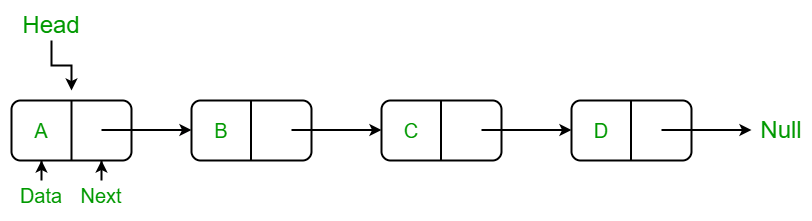
\includegraphics[width=0.8\linewidth]{photo/linkedlist.png}
\end{figure}

\subsubsection{Liste con puntatore doppio}


Una lista a puntatore doppio è una struttura dati dinamica che consiste di una sequenza di nodi, ognuno dei quali contiene un campo di dati e due riferimenti, uno al nodo precedente e uno al nodo successivo. 
\\
Quindi la struttura della lista sarà:
\begin{lstlisting}[language=C]
typedef struct node{
	struct node *prev; \\contiene il puntatore all'elemento precedente
	int data;
	struct node *next; \\contiene il puntatore all'elemento successivo
}Node;
\end{lstlisting}

\begin{figure}[h]
	\centering
	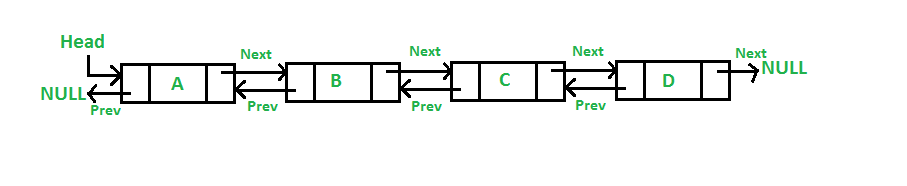
\includegraphics[width=0.7\linewidth]{photo/DLL}
\end{figure}
\newpage
Ecco alcuni esempi di operazioni che possono essere eseguite su una lista a puntatore doppio:
\begin{itemize}
\item \textbf{Inserimento di un elemento}: Per inserire un elemento alla fine della lista, è sufficiente creare un nuovo nodo e collegarlo al nodo finale. Per inserire un elemento all'inizio della lista, è necessario collegare il nuovo nodo al nodo iniziale
\begin{lstlisting}[language=C]
 void insert_at_head(list_node **head, int value) {
 	// Crea un nuovo nodo
 	list_node *new_node = malloc(sizeof(struct list_node));
 	new_node->value = value;
 	
 	// Collega il nuovo nodo al nodo iniziale
 	new_node->next = *head;
 	new_node->prev = NULL;
 	
 	// Collega il nodo iniziale al nuovo nodo
 	if (*head != NULL) {
 		(*head)->prev = new_node;
 	}
 	*head = new_node;// Imposta il nuovo nodo come nodo iniziale
 }
\end{lstlisting}
\item \textbf{Eliminazione di un elemento}:Per eliminare un elemento dalla lista, è sufficiente scollegare il nodo desiderato dai nodi adiacenti.
\begin{lstlisting}[language=C]
	void delete_element(struct list_node **head, int value) {
		// Trova il nodo da eliminare
		struct list_node *node = *head;
		while (node != NULL && node->value != value) {
			node = node->next;
		}
		
		// Controlla se il nodo e' stato trovato
		if (node == NULL) {
			return;
		}
		
		// Scollega il nodo dai nodi adiacenti
		if (node->prev != NULL) {
			node->prev->next = node->next;
		}
		if (node->next != NULL) {
			node->next->prev = node->prev;
		}
		
		// Libera la memoria allocata per il nodo
		free(node);
	}
	
\end{lstlisting}
\item \textbf{Ricerca di un elemento nella lista}:Per cercare un elemento nella lista, è possibile utilizzare un iteratore per navigare attraverso la lista fino a trovare l'elemento desiderato.
\begin{lstlisting}[language=C]
	int cerca(int n,nodo* head){
		int posizione = -1;
		int trovato = 0;
		int i=0;
		while(head != NULL && trovato == 0){
			if(head -> elemento == n){
				posizione = i;
				trovato = 1;
			}
			i++;
			head = head -> successivo;
		}
		return posizione;
	}
\end{lstlisting}
\end{itemize}
\newpage
\subsection{Pile}
Una pila è un particolare tipo di lista in cui gli inserimenti e le cancellazioni avvengono ad un estremo della struttura , ovvero:
\begin{itemize}
\item Gli inserimenti avvengono solo dopo l'ultimo elemento 
\item La cancellazione avviene solo sull'ultimo elemento
\end{itemize}
Generalmente le liste utilizzano il principio di \verb*|LIFO| (Last In First Out), ovvero l’elemento inserito per ultimo è il primo elemento a uscire dalla lista.

\begin{figure}[h]
	\centering
	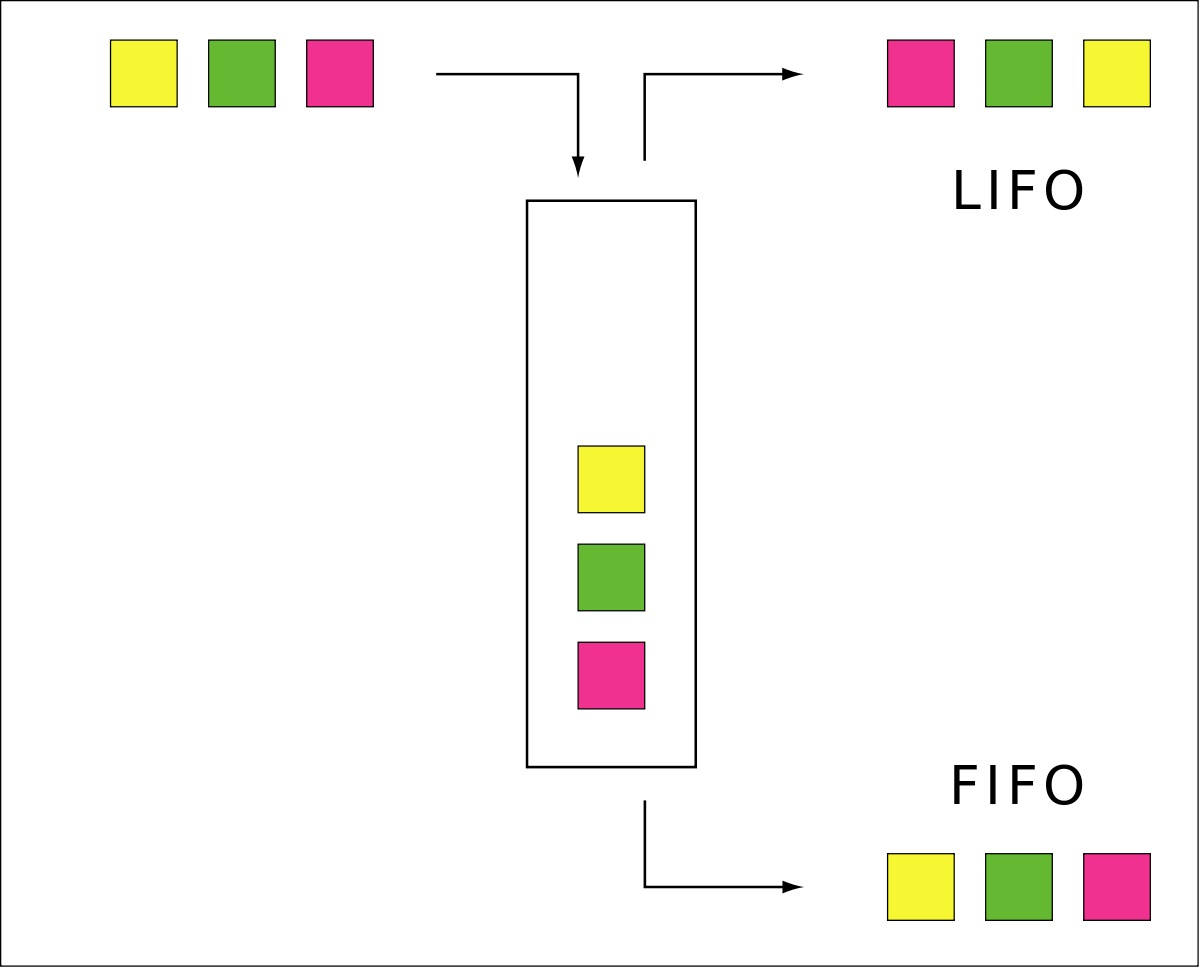
\includegraphics[width=0.5\linewidth]{photo/lifovsfifo}
\end{figure}
Funzioni classiche quando si ha a che fare con le pile sono:
\begin{itemize}
	\item \verb|push(P,v)| per l'operazione di inserimento 
	\item \verb*|pop(P)| per l'operazione di cancellazione del primo elemento(pop restituisce il contenuto dell'elemento cancellato)
	\item \verb*|top(P)| per l'operazione che legge l'ultimo elemento in cima alla pila
\end{itemize}
\subsection{Code}
il tipo di dato coda è una specializzazione della lista in cui: 
\begin{itemize}
\item 	Gli eventi di inserimento avvengono solo all'estremo della lista(prima dalla testa, o dopo la coda)
\item Gli eventi di cancellazione avvengono solo all'altro estremo (alla coda, oppure alla testa)
\end{itemize}
Le procedure per l'inserimento e la rimozione di un dato dato il contesto prendono il nome:
\begin{itemize}
	\item \verb*|enqueue(Q,v)| per l'operazione di inserimento
	\item \verb*|dequeque(Q)| per l'operazione di cancellazione (che restituisce il contenuto dell'elemento cancellato)
\end{itemize}
\begin{figure}[h]
	\centering
	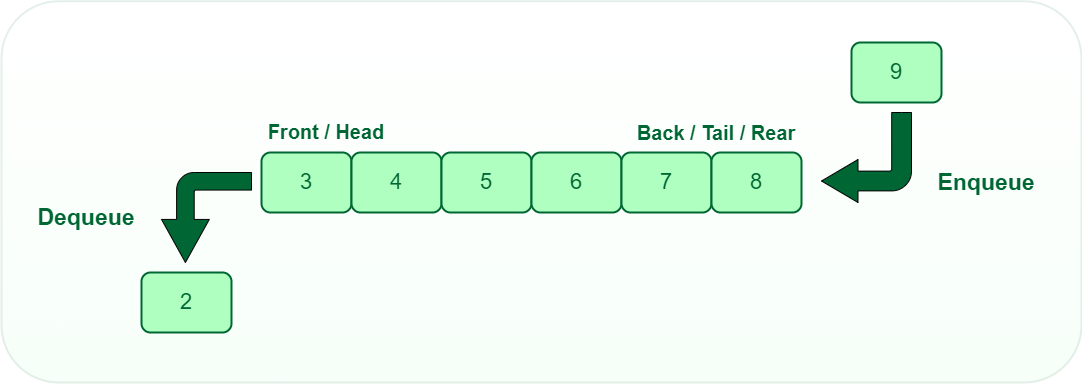
\includegraphics[width=0.7\linewidth]{photo/Queue}
\end{figure}
\newpage
\subsection{Strutture ad albero}
Un albero è una struttura dati gerarchica che consiste di nodi collegati tra loro da archi. Ogni nodo(tranne la radice) ha uno e un solo padre e può avere zero o più nodi figli. Il nodo senza figli è chiamato nodo foglia.
\begin{figure}[h]
	\centering
	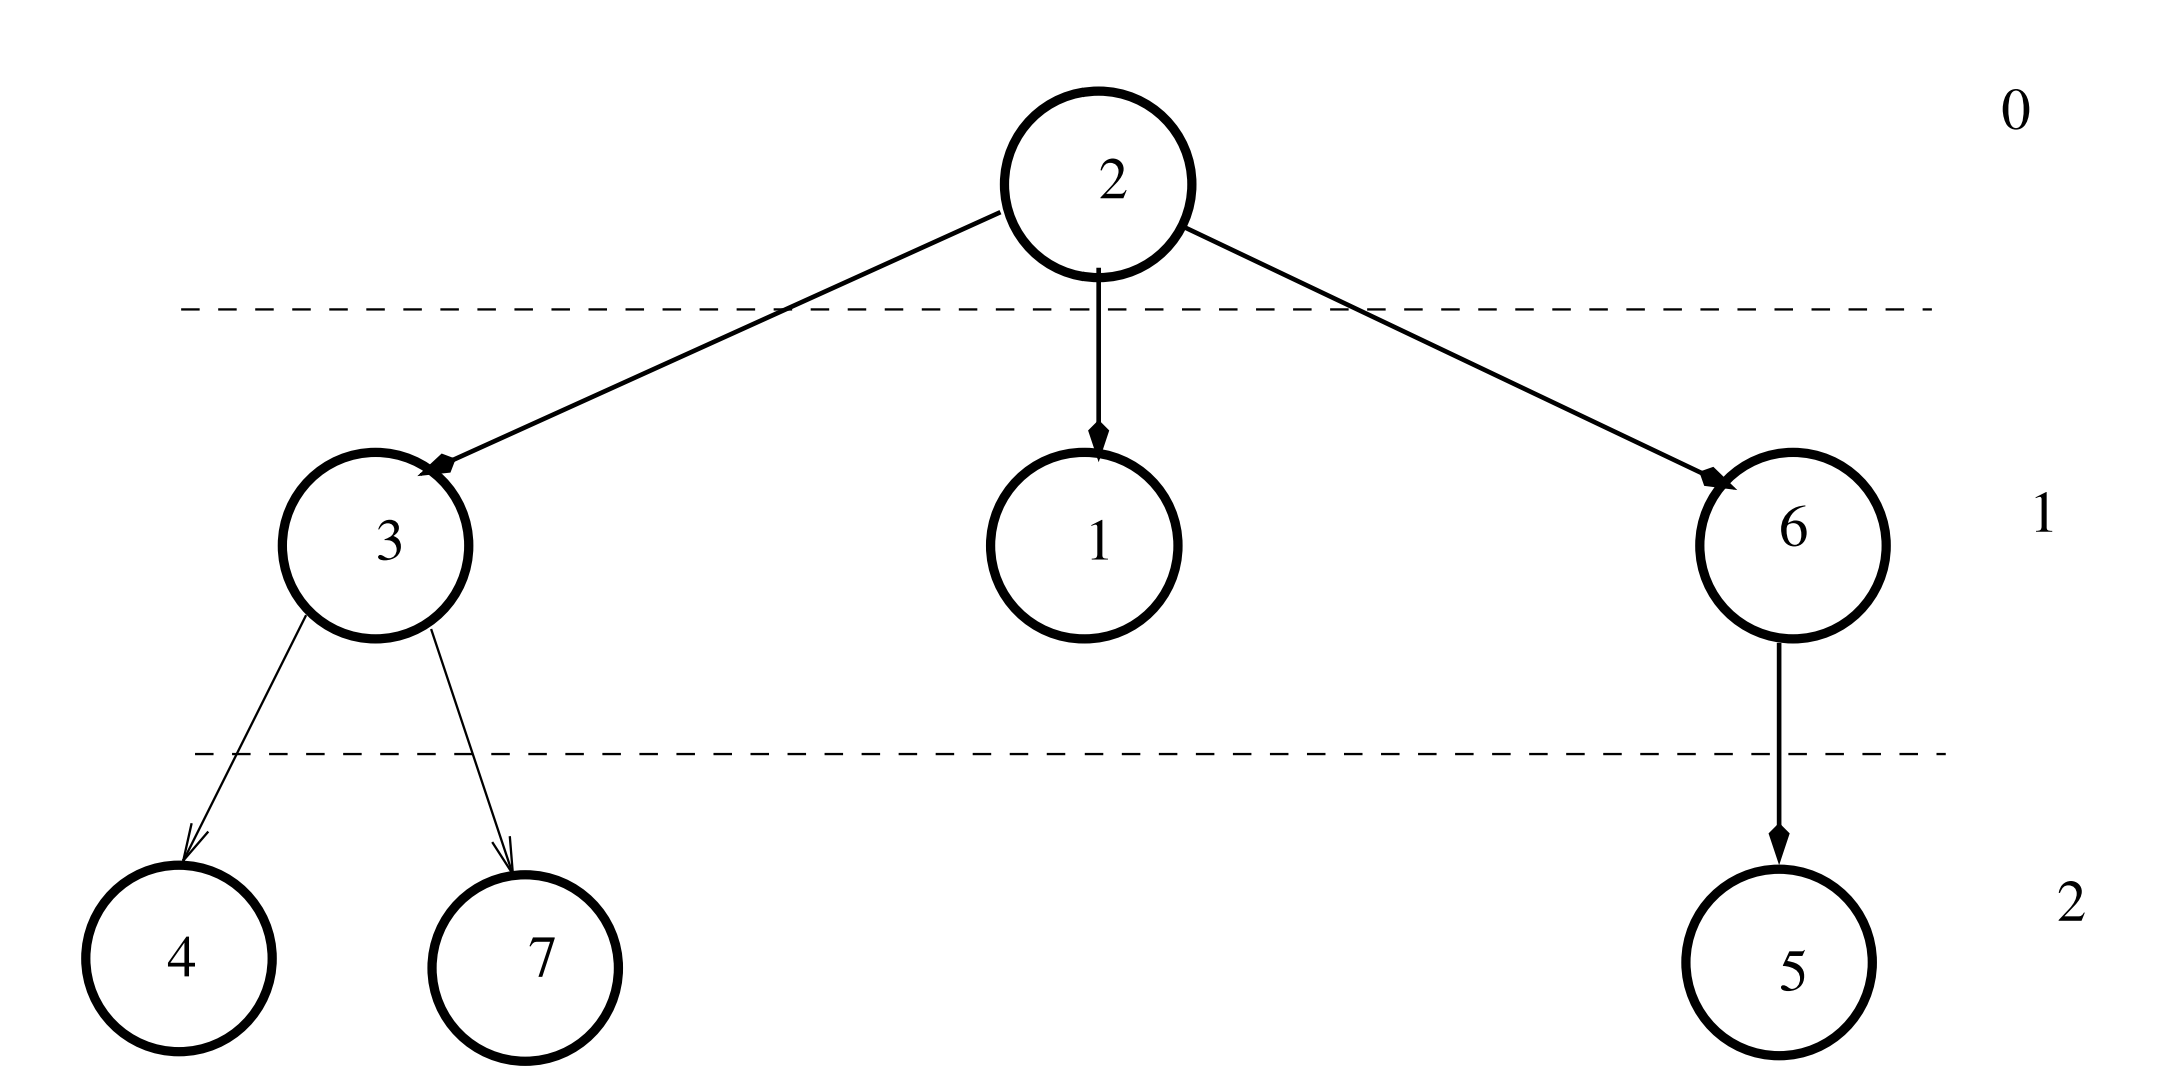
\includegraphics[width=0.6\linewidth]{photo/albero}
\end{figure}

\textbf{Profondità dei nodi}: è la lunghezza del cammino semplice della radice al nodo(misurato in numero di archi)
\\
\textbf{Ex.}: la radice ha profondità 0, i suoi figli hanno profondità 1 e i figli dei figli hanno profondità 2
\\
\\
\textbf{Livello}: l'inseme dei nodi alla stessa profondità \\
\\
\textbf{Altezza albero}:La profondità massima delle sue foglie.
\subsubsection{Albero binario}
Un albero binario è un albero radicato in cui ogni nodo ha al massimo due figli, identificati come figlio destro e figlio sinistro.
\subsubsection{Alberi binari di ricerca}
Un albero binario di ricerca (BST) è una struttura dati gerarchica in cui ogni nodo può avere al massimo due figli. I figli di un nodo sono chiamati figlio sinistro e figlio destro.
\\
\\
In un BST, i valori dei nodi sono ordinati in modo crescente. Ciò significa che il valore di ogni nodo è maggiore o uguale al valore del suo figlio sinistro e minore o uguale al valore del suo figlio destro.
\\
\\
Gli alberi binari di ricerca sono spesso utilizzati per implementare algoritmi di ricerca efficienti, come la ricerca binaria. La ricerca binaria funziona confrontando il valore dell'elemento da cercare con il valore del nodo radice. Se i due valori sono uguali, l'elemento è stato trovato. In caso contrario, il valore viene confrontato con il valore del figlio sinistro o del figlio destro del nodo radice, a seconda di quale dei due valori sia minore. Il processo viene ripetuto fino a quando l'elemento viene trovato o fino a quando viene raggiunto un nodo foglia, che indica che l'elemento non è presente nell'albero.

\subsubsection{Alberi bilanciati}

La bilanciatura di un albero binario di ricerca (BST) consiste nel mantenere la struttura dell'albero in modo tale che la profondità di ogni nodo sia il più vicina possibile alla profondità media dell'albero. Ciò migliora l'efficienza delle operazioni di ricerca e inserimento, che sono operazioni \( O(log\: n) \) in un BST bilanciato.
\\
\\
Esistono diversi tipi di alberi bilanciati: 
\begin{itemize}
\item\textbf{ Alberi AVL} : Gli alberi AVL sono BST bilanciati in cui la differenza tra la profondità dei sottoalberi sinistro e destro di ogni nodo non supera mai 1. Gli alberi AVL sono facili da implementare e hanno prestazioni eccellenti.
\item  \textbf{B-alberi}: Un B-albero (in inglese: B-tree) è una struttura dati che permette la rapida localizzazione dei file (record o chiavi), specie nelle basi di dati, riducendo il numero di volte che un utente necessita per accedere alla memoria in cui il dato è salvato.
\item \textbf{Alberi 2-3}: Gli alberi 2-3 sono BST bilanciati in cui ogni nodo può avere al massimo due figli, uno sinistro e uno destro. I nodi interni degli alberi 2-3 possono contenere al massimo due valori.
\item \textbf{Alberi rosso - neri}:Gli alberi rosso-neri sono un tipo di albero binario di ricerca (BST) bilanciato. Gli alberi rosso-neri soddisfano le seguenti proprietà:
\begin{itemize}
	\item Ogni nodo è rosso o nero.
	\item La radice dell'albero è nera.
	\item Tutti i fogli (nodi senza figli) sono neri.
	\item Se un nodo è rosso, entrambi i suoi figli devono essere neri.
	\item Ogni percorso da una foglia alla radice contiene lo stesso numero di nodi neri.
\end{itemize}
Queste proprietà garantiscono che l'altezza di un albero rosso-nero sia sempre \( O(log\: n) \), dove n è il numero di nodi dell'albero.
\end{itemize}
\begin{figure}[h]
	\centering
	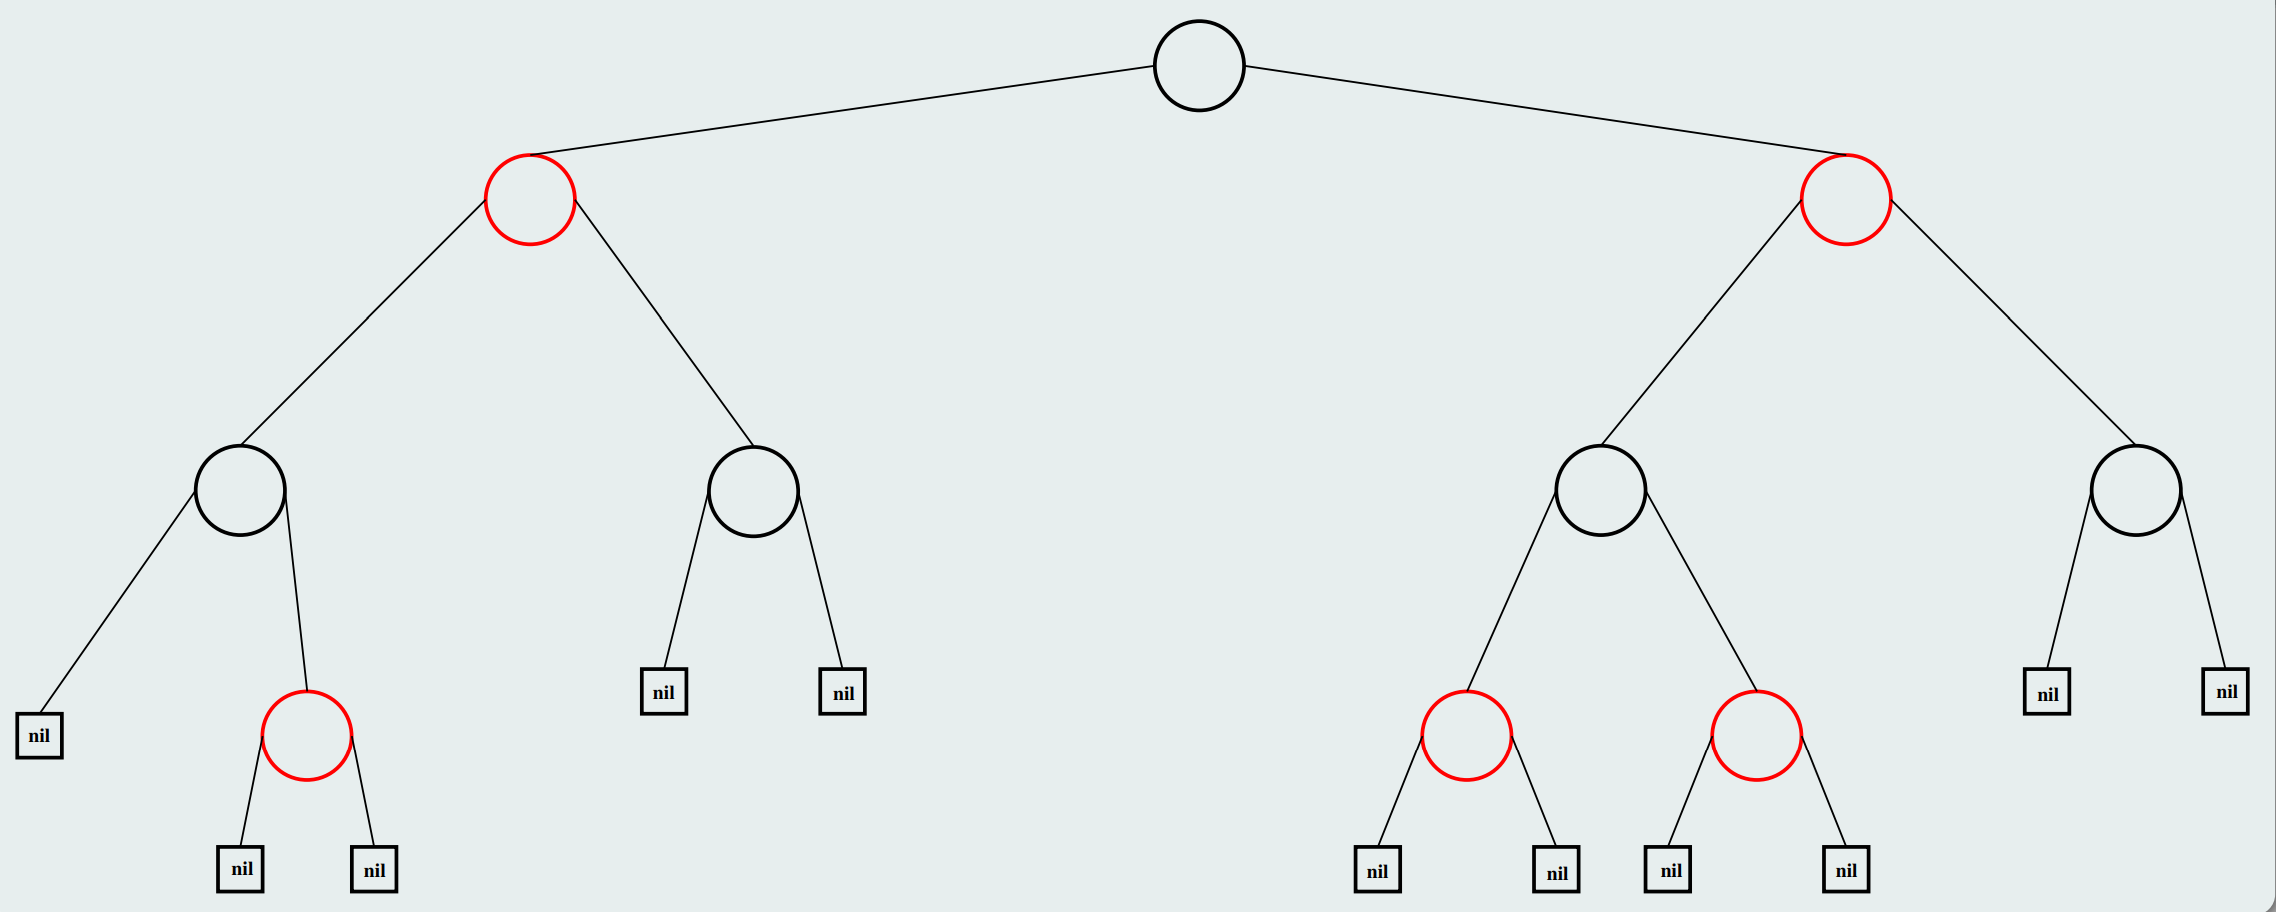
\includegraphics[width=0.8\linewidth]{photo/alberoRN}
\end{figure}

\end{document}

